%\RequirePackage[l2tabu, orthodox]{nag}  %Checks for older packages 

\documentclass[11pt,a4paper]{article}
% \documentclass[10pt]{extreport} $ allos to make the font smaller
\usepackage[utf8]{inputenc}

\usepackage{amsmath}
\usepackage{amsfonts}
\usepackage{indentfirst}
\usepackage{amssymb}
\usepackage{siunitx}  % Units of the metric system  \SI{2.63}{\ohm}   
\usepackage[font={footnotesize}]{caption} %Makes the captions small

\usepackage{algorithm}
\usepackage{algpseudocode}

%% Figures packages
\usepackage[pdftex]{graphicx}
\usepackage{float}   %Es para colocar el objeto flotante exactamente donde se ponga el comando con H
\usepackage{caption}
\usepackage{subcaption}
\graphicspath{{../results/}}
\usepackage{sidecap}  %Para poner figuras a los lados


\usepackage{setspace} % Needed for Pyton syntax highlight
\usepackage{listings}    % Include the listings-package, nice verbatim for code
\usepackage{color}
\usepackage{courier}


\usepackage{cleveref} %puts figure and equation appropiately \cref{} 

\usepackage{natbib} %For bibliography
%\usepackage{cite}
\usepackage{framed} % To use boxes, or frames around text

\usepackage{parskip} %Para saltos entre parrafos
\setlength{\parindent}{0pt} 
\setlength{\parskip}{\baselineskip}
\usepackage[a4paper,margin=0.8in]{geometry}  %%Cambiar los margenes

\newcommand{\HRule}{\rule{\linewidth}{0.5mm}}

%\usepackage{hyperref} %This should be loade after most of the other packages 
% \hypersetup{colorlinks=true}  %Para que los hiperlinks cuando se hagan referencias aparezcan en colores.



\definecolor{dkgreen}{rgb}{0,0.6,0}

\title{Lab12: DD2380 }
\author{
Ramon Heberto Martinez Mayorquin  hramon@kth.se 
Akash Kumar Dhaka  akashd@kth.se 
}



\begin{document}

\begin{titlepage}
\begin{center}
%\includegraphics[width=0.15\textwidth]{logo}\\[1cm]    

\textsc{\LARGE Kungliga Tekniska högskolan}\\[1.0cm]

\textsc{\Large Summer School: Introduction to High Performance Computing}\\[2.0cm]



\begin{figure}[H]
	\centering
 
\includegraphics[width=0.35\textwidth]{Kth_logo.png}
\end{figure}
%\\[1cm]    
%

% Title
\HRule \\[0.4cm]
{ \huge  Project: Stochastic Gradient Descent in CUDA.
}\\[0.4cm]
\HRule \\[1.5cm]

% Author and supervisor

Authors: Ram\'on  Mart\'inez, Theodore Vasiloudis   \\ 
\large Professors: One Dude, The other dude.  \\ [2.5cm]
%\normalsize Presenta \\
%\large Supervisors 2: Jan Antolik \\[2.5cm]

\textsc{\Large School of Computer Science and Communication \\
PDC Center for High Performance Computing}\\ [1.0cm] 
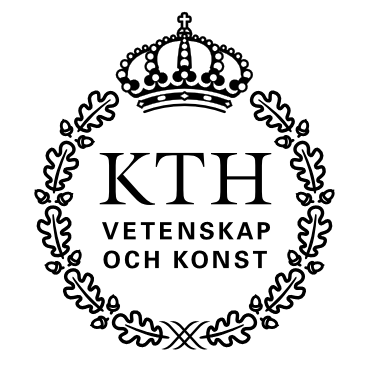
\includegraphics[width=0.15\textwidth]{KTH_black.png}\\[1.5cm] % Controls the distance till the new object 
% Bottom of the page
{\large 15 September of 2015}

\end{center}
\end{titlepage}

\begin{abstract}
Parallelize this parallelize that.

\end{abstract}

\section{Stochastic Gradient Descent}


One of the most common problems in machine learning, estimation and optimization theory is the one of minimizing an objective function \citep{bottou2010large}. Consider the \textit{loss} function $Q(z, w)$. This function depends both of the sample $z=(x, y)$ which is a pair of input $x$ and output $y$ and on the vector $w$ which parametrizes the function that connects the input to the output. In such a context we will like to find the vector $w$ that minimizes this error averaged over the sample. Or in a more mathematical parlance the following statement:

\begin{equation}
E(w) = \frac{1}{n} \sum_{i=1}^n Q(z_i, w)
\end{equation}

Where the index $i$ goes through all the samples $z$. 

The general method of Gradient Descent proposes moving in the direction of the gradient in order to find $w$. 

\begin{equation}
w_{t + 1} = w_t - \gamma \sum_{i=1}^n \triangledown_w Q(z_i, w)
\end{equation}

Where $gamma$ is called the usually called the learning rate and controls the speed of convergence (or divergence if it is too big). 

Under sufficient regularity assumptions when the initial estimate of $w$ is close enough to the minimum and the learning rate is small enough this algorithm can achieve linear convergence \citep{dennis1996numerical}. 

Stochastic Gradient Descent is a simplification of the scheme proposed above. In this case the average over the sample space is put aside and instead we use the local gradient to indicate the proper direction of movement:

\begin{equation}
w_{t + 1} = w_t - \gamma  \triangledown_w Q(z_i, w)
\end{equation} 

It follows from the algorithm that this optimazation can be implemented online due to the fact that not memory is needed no the calculation. The convergence of stochastic gradient descent is granted in some mild conditions when the learning rate $gamma$ decreases over time in such a way that the series indexed by them does not diverge \citep{bottou2010large}. 

It is the general wisdom that when the learning samples form a big set (big data) Stochastic Gradient Descent can achieve a better performance that its normal version. There is research, however, that points out the domain of application of this method is greater and overall surpasses Gradient Descent in most of domains \citep{wilson2003general}. 

\bibliographystyle{plainnat}
\bibliography{references}
\end{document}